\section{Design}

\subsection{Component Division}

The first question that has to be answered is whether or not it makes sense to divide the bootware component into two or more cooperating components, i.e. a server client division or a similar structure.
As described in \autoref{related:ondemand} on page \pageref{related:ondemand}, the proposed architecture initially only envisioned one bootware component.
This architecture was expanded with the introduction of the provisioning manager, as described in \autoref{related:dynamic} on page \pageref{related:dynamic}.
We will now discuss the viability of these architectures.b

\subsubsection{Single Local Component}

\begin{figure}[!htbp]
	\centering
	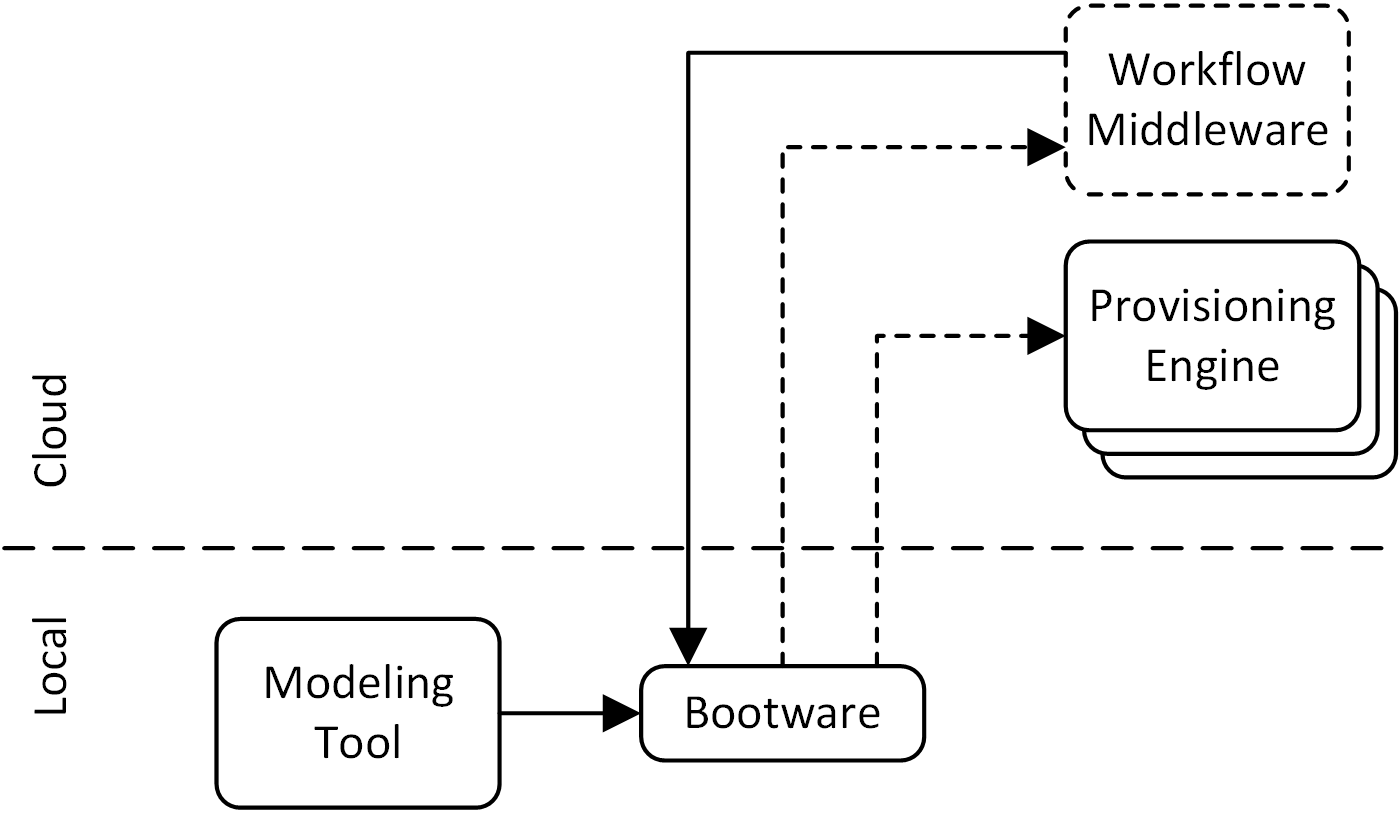
\includegraphics[resolution=600]{design/assets/simple_local}
	\caption{Simplified overview of the single local component architecture}
	\label{image:single_local}
\end{figure}

First we consider the simplest case: A single local component.
In this scenario, all provisioning processes are initiated from a component installed locally on the users machine, alongside or as part of the workflow modeler.

The advantages of this architecture lie in its simplicity.
Only one component has to be created and managed.
There is no possible overlap in functionality, as in a 2-tier architecture (see \autoref{design:division:2tier}.
Communication between multiple bootware components doesn't have to be considered.

The disadvantages are caused by the component being local.
Since all the functionality is concentrated in one component, it can become quite large and complicated, is is one thing that should be avoided according to the requirements.
A much bigger problem however is the remote communication happening in this scenario.
All calls to the bootware component from the ESB of the workflow middleware would leave the remote environment.
Also, all calls from the bootware component to the provisioning engines would enter the remote environment.
This type of split communication can be costly and slow \textcolor{red}{(add source/description)}.

\subsubsection{Single Remote Component}

\begin{figure}[!htbp]
	\centering
	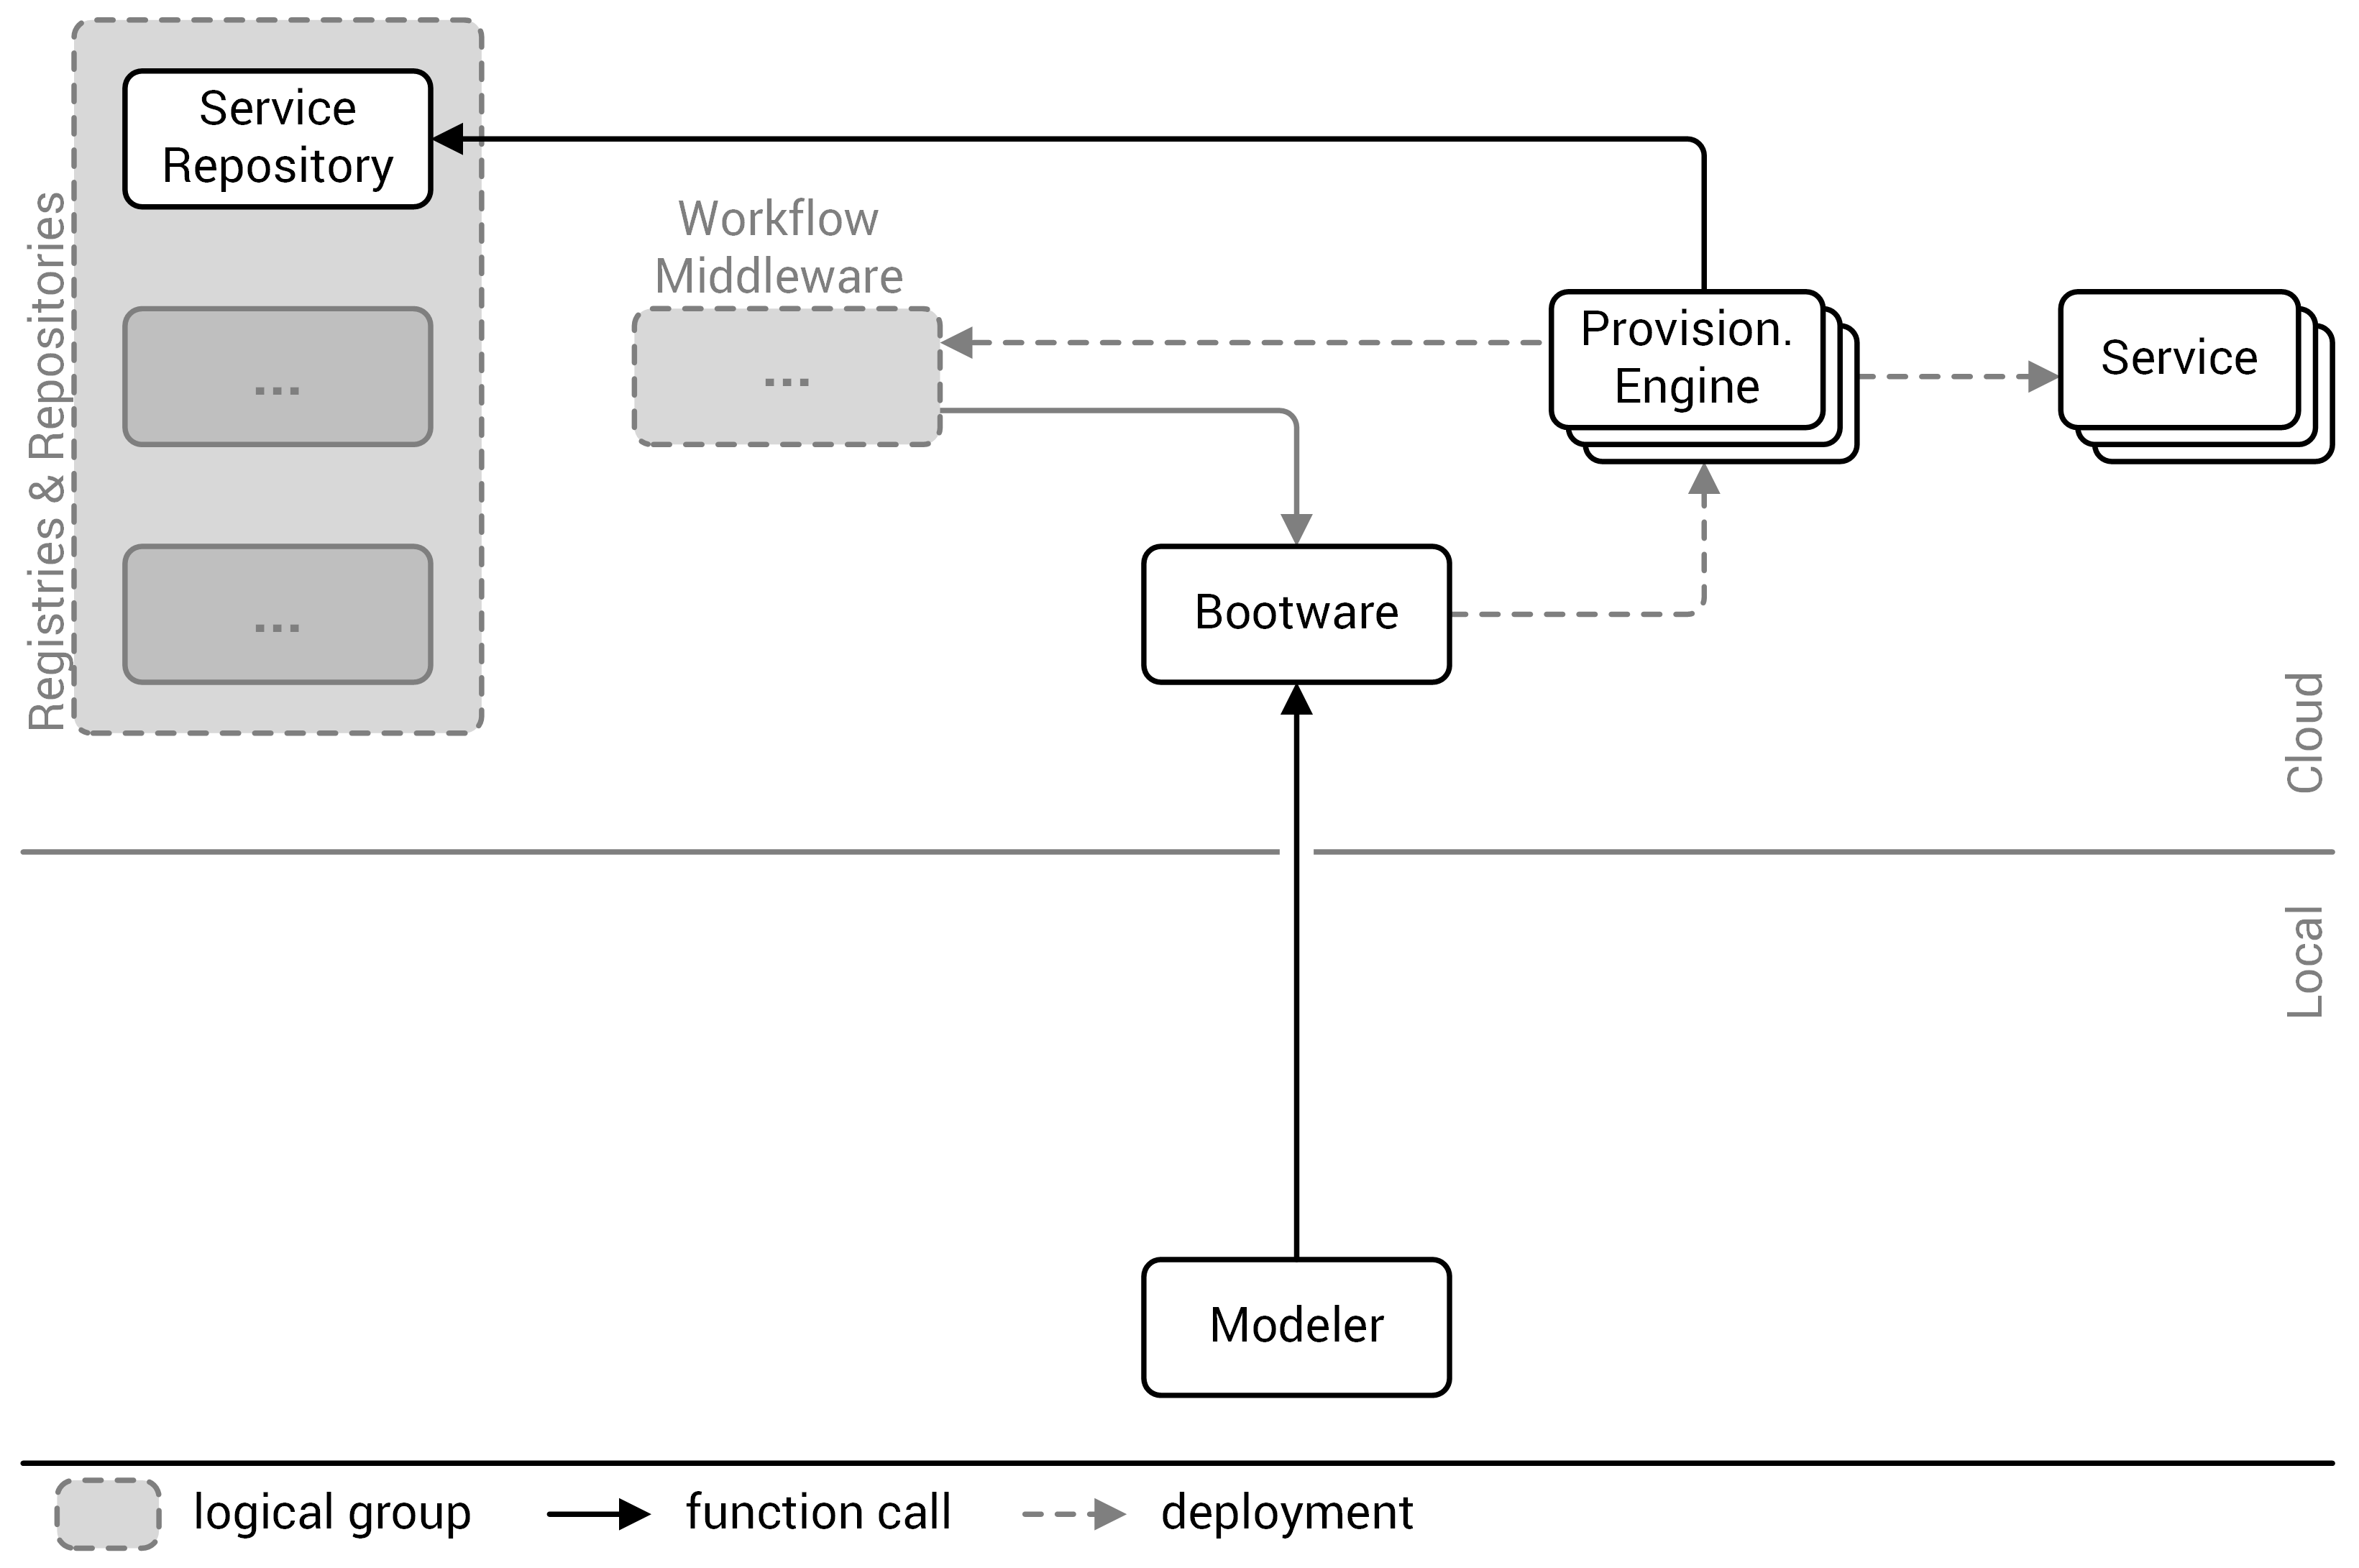
\includegraphics[resolution=600]{design/assets/simple_remote}
	\caption{Simplified overview of the single remote component architecture}
	\label{image:single_remote}
\end{figure}

The next obvious choice is to put the single bootware component into a remote environment, where the disadvantages of local to remote communication would disappear.

However, this creates a new problem.
We don't know where exactly to put the bootware component.
Since one requirement is that multiple cloud environments should be supported, it's possible that the bootware component is not located anywhere near the cloud environment where it should provision further components.
The communication problem of the single local bootware component still exist.

Another problem is that now we would have to manage some sort of load balancing and the bootware component would have to support multiple tenancy or be stateless, or otherwise every user needs its own remote instance.
The first case would further complicate the design and implementation of the bootware component.
The second case would increase monetary and management costs.

\subsubsection{2-Tier Architecture}
\label{design:division:2tier}

\begin{figure}[!htbp]
	\centering
	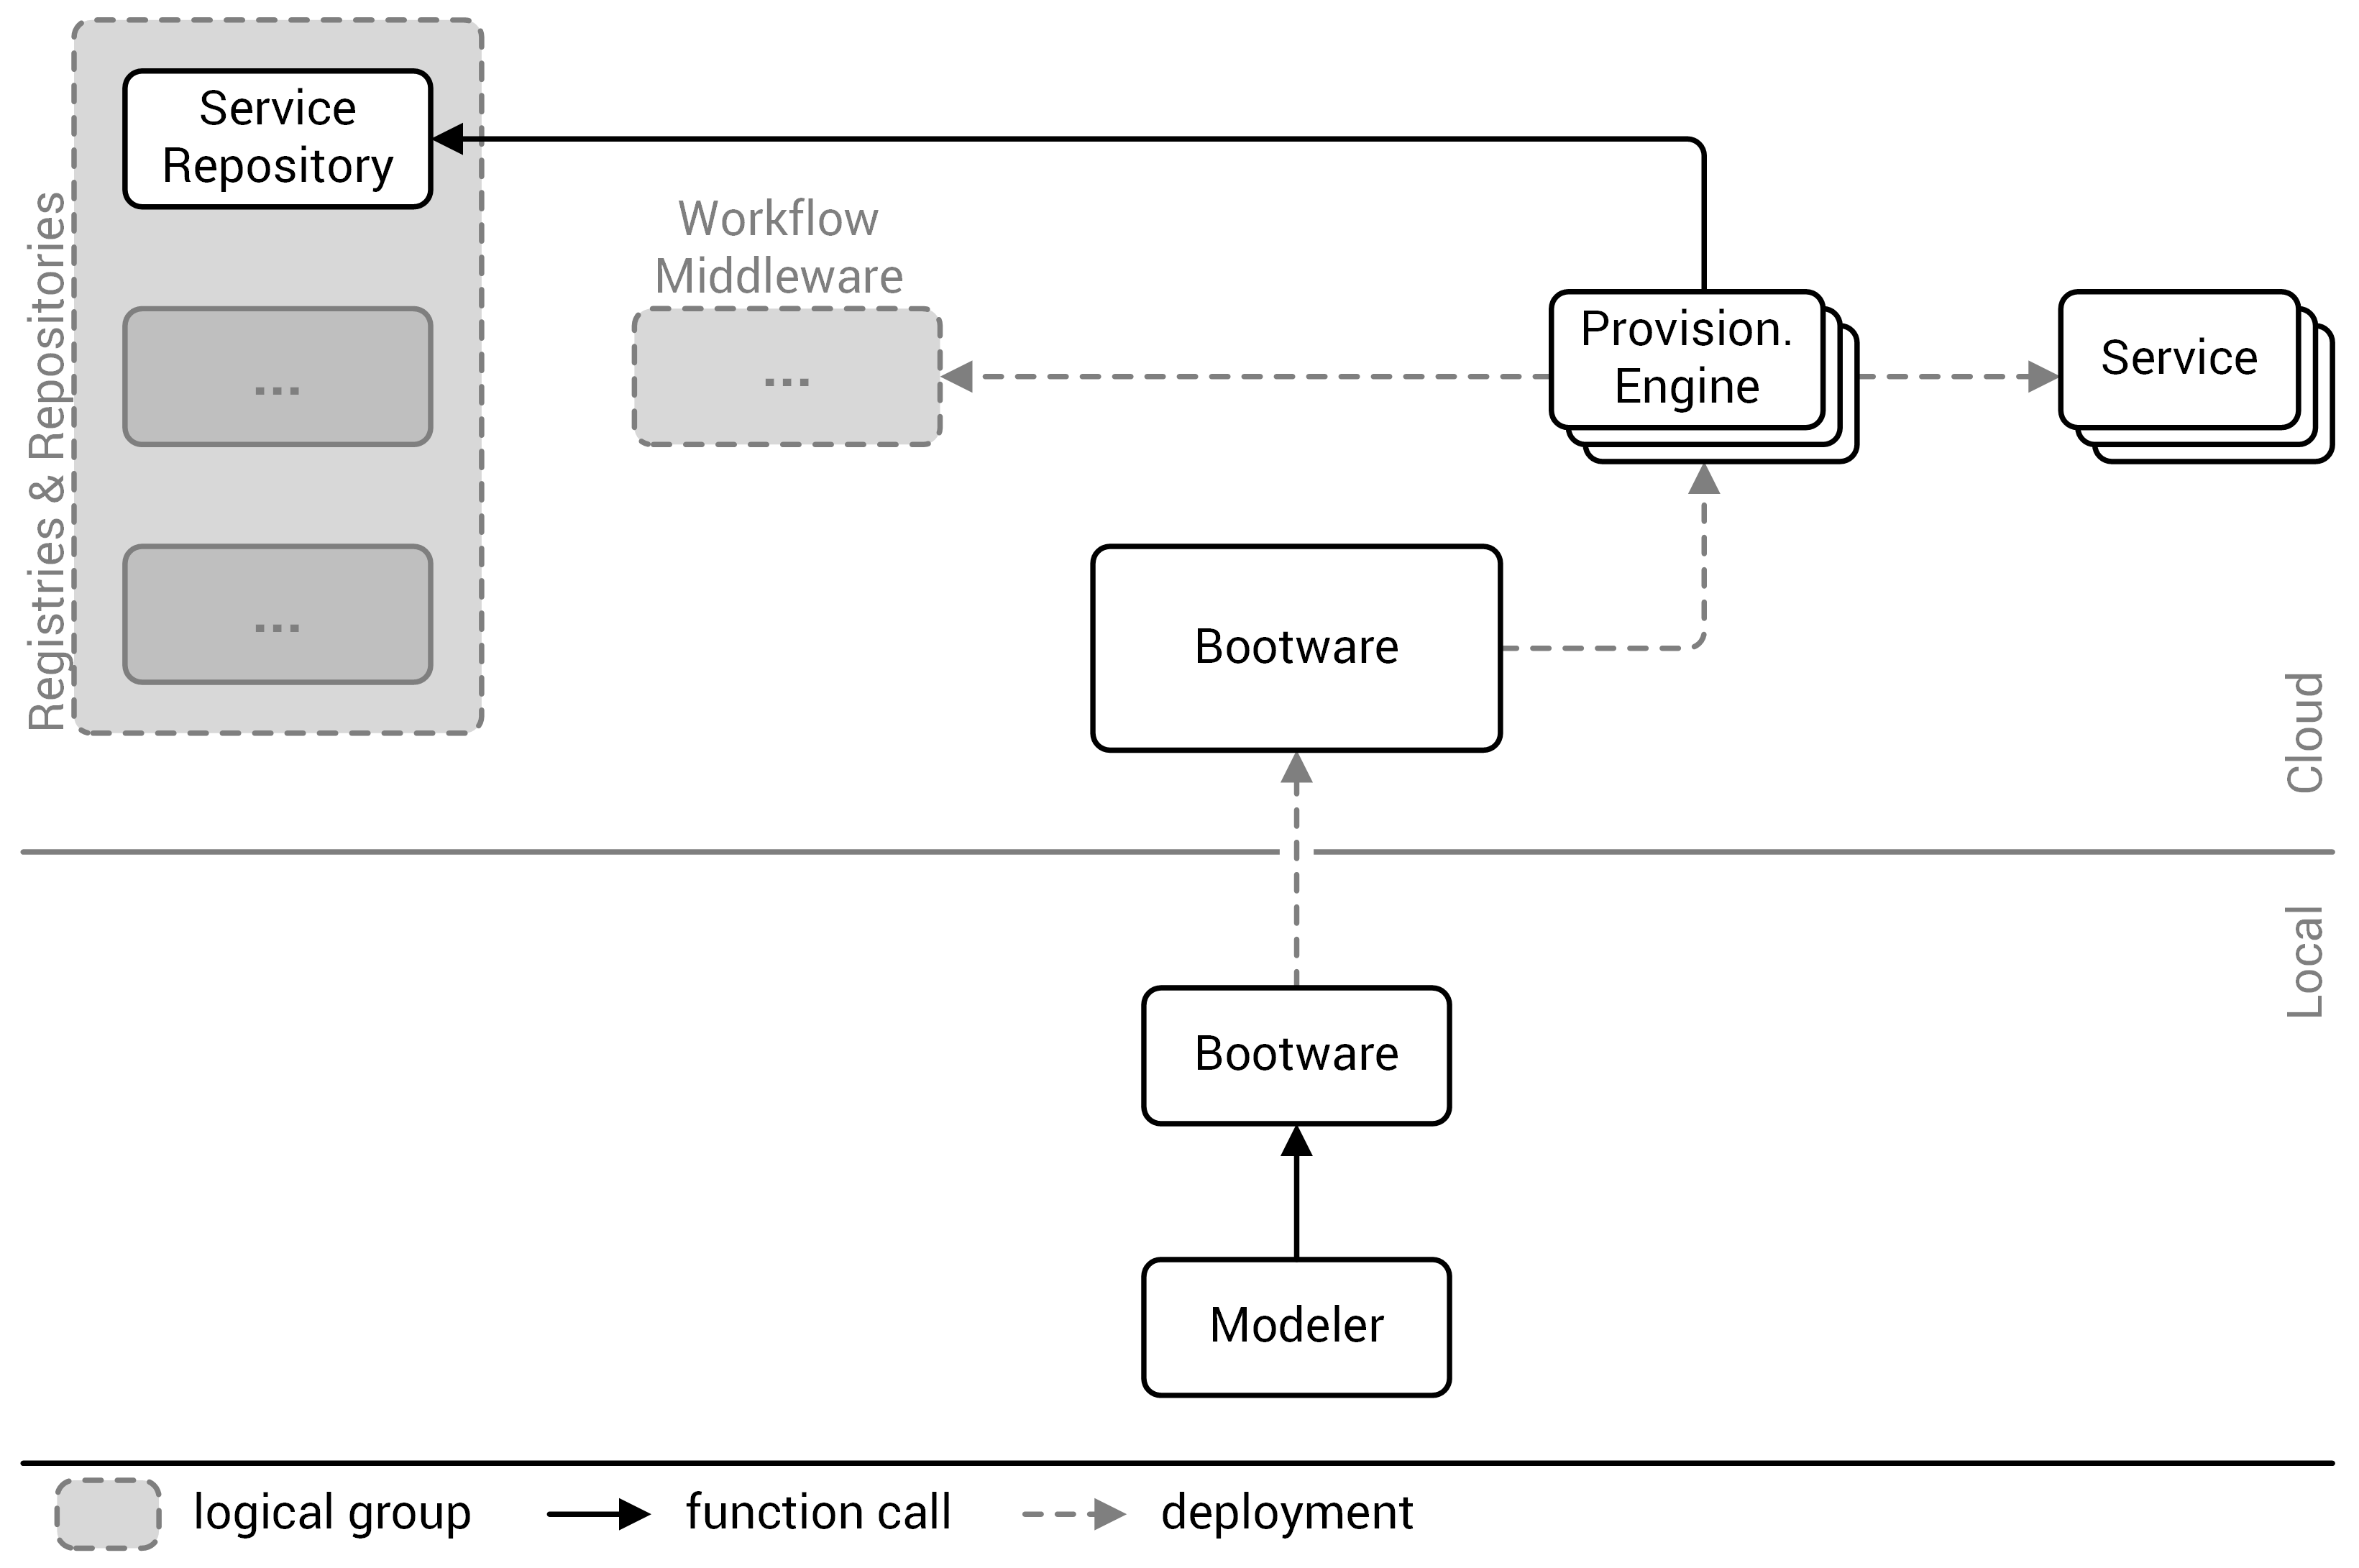
\includegraphics[resolution=600]{design/assets/simple_2_tier}
	\caption{Simplified overview of the 2-tier architecture}
	\label{image:single_2_tier}
\end{figure}

Next, we take a look at a 2-tier architecture, where the bootware is divided into two components.
On the local side we have a small and simple component which has mainly one function: To provision the larger second part of the bootware in a remote environment near to the environment, where other components will be provisioned later.

This eliminates the problems of a single bootware component.
We can now keep the local part as simple as possible and make the remote part as complicated as it has to be.
We now also can position the remote component close to other remote components to minimize local/remote communication and the problems resulting of it.

But we also introduce new problems.
For one, we now have duplicate functionality between the two components.
Both components have to know how to provision a component into multiple cloud environments.
The local component has to be able to put its remote counterpart into any cloud environment.
The remote component has to be able to provision other components into the same environment in which it runs (ideally, to minimize costs).
Since itself can be located in any cloud environment, it has to be able to do this in any cloud environment.
Independent from this, it has to be able to provision to any environment that the user/service package chooses.
But this problem can be solved by using a plugin architecture, which allows both components to use the same plugins.
We discuss plugins in detail in \autoref{design:extensibility}.

A second problem which we can't avoid but can solve is the communication which is now necessary between the different parts of the bootware.
More on this in \autoref{design:communication}

\subsubsection{Cloning}

\begin{figure}[!htbp]
	\centering
	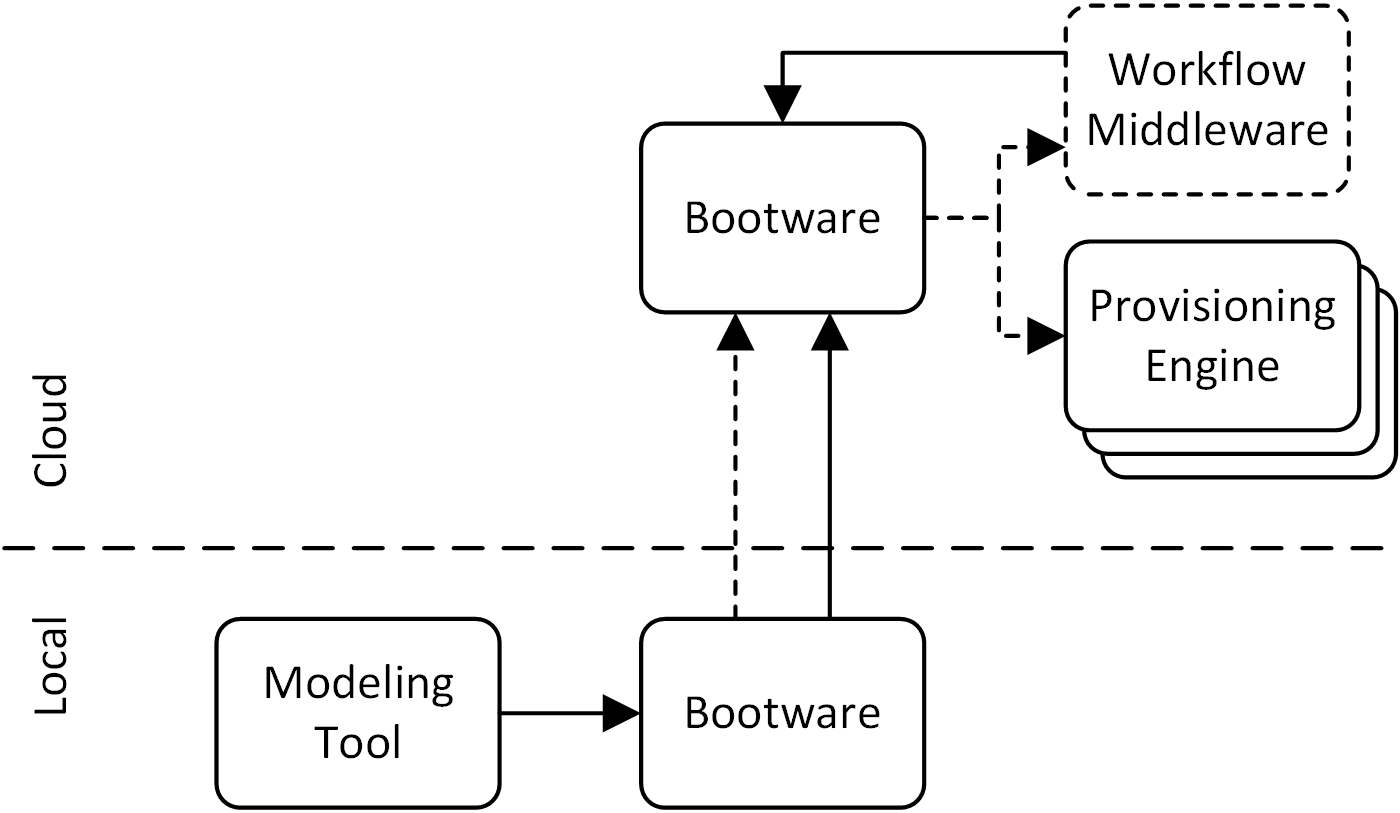
\includegraphics[resolution=600]{design/assets/simple_clone}
	\caption{Simplified overview of the cloned component architecture}
	\label{image:single_clone}
\end{figure}

This architecture can be seen as an alternative form of the 2-tier architecture described in \autoref{design:division:2tier}.
In this case there are also two parts working together and the remote part does the most of the work.
However, the local and the remote components are identical.
Instead of provisioning a bigger component in a remote environment, the local component clones itself.
Compared to the 2-tier architecture described before, this has the advantage that only one component has to be designed and implemented and that function duplication is not an issue.
On the other hand, this architecture makes only sense if the functionality of the two separate components in the 2-tier architecture turns out to be mostly identical.
Therefore we can't decide yet if this architecture should be used.

\textcolor{red}{Decide on one architecture}

\subsection{Extensibility}
\label{design:extensibility}

The requirements for the bootware component state that support for different cloud environments and provisioning engines should be achieved through means of software engineering.
This requirement is intentionally vague to allow to select a fitting extension mechanism during the design process.

\textcolor{red}{other mechanisms?}

One possibility that would satisfy this criteria is to design interfaces for all extension points of the bootware component.
New cloud environments, provisioning engines, or other extension could then implement these interfaces.
The disadvantage of this approach is that the whole bootware component has to be recompiled, redistributed and redeployed if one extension is added or changed.

To remove this disadvantage, a more flexible architecture is needed, for example a plugin architecture. (textcolor{red}{pattern?})
Interfaces for the extension points still exist but the extension are no longer part of the main bootware component.
They are compiled separately into plugins that can be loaded into the main bootware component on the fly.
There are several possibilities to realize such an architecture.

It is certainly possible to implement a plugin framework from scratch.
An advantage of this approach would be that the design of the plugin architecture could be tailored to our use case and would be as simple or complex as needed.
But there are also several disadvantages.
For one, we would reinvent the wheel, since multiple such frameworks already exist.
It would also shift resources away from the actual goal of this thesis, which is designing the bootware component.
Furthermore it would require a deep understanding of the language used for the implementation (\textcolor{red}{in this case Java}), which is not necessarily given.
Therefore it seems more reasonable to use one of the already existing plugin frameworks.Three such alternatives will be compared next. (\textcolor{red}{more?})

\begin{savenotes}
\begin{table}[!htpb]
	\centering
	\small
	\begin{tabular}{rl|ccc}

		&
		& \multicolumn{3}{c}{\textit{Plugin Frameworks}} \\

		&
		& \begin{sideways} \textbf{JSPF\footnote{\url{https://code.google.com/p/jspf/}\label{jspf}}} \end{sideways}
		& \begin{sideways} \textbf{JPF\footnote{\url{http://jpf.sourceforge.net/}\label{jpf}}} \end{sideways}
		& \begin{sideways} \textbf{OSGi\footnote{\url{http://www.osgi.org/}\label{osgi}}} \end{sideways} \\

		\cline{2-5}

		\multirow{7}{*}{\textit{Features}}

		& \textbf{Security}
		& \ding{55}    % jspf
		& \ding{55}    % jpf
		& \ding{51} \\ % osgi

		& \textbf{Dynamic Loading}
		& \ding{55}    % jspf
		& \ding{51}    % jpf
		& \ding{51} \\ % osgi

		& \textbf{Complexity}
		& low     % jspf
		& medium  % jpf
		& high \\ % osgi

		& \textbf{Active Development}
		& \ding{55}    % jspf
		& \ding{55}    % jpf
		& \ding{51} \\ % osgi

		& \textbf{Popularity}
		& low     % jspf
		& low     % jpf
		& high \\ % osgi

		& \textbf{Standard}
		& \ding{55}    % jspf
		& \ding{55}    % jpf
		& \ding{51} \\ % osgi

		& \textbf{Used in SimTech}
		& \ding{55}    % jspf
		& \ding{55}    % jpf
		& \ding{51} \\ % osgi

		\cline{2-5}

		% \multirow{2}{*}{\pbox{2cm}{\vspace{0.9em} \textit{Application} \\ \textit{Servers}}}

	\end{tabular}
	\caption{Feature comparison of Java plugin frameworks}
	\label{table:plugin_comparison}
\end{table}
\end{savenotes}

All of the frameworks that we compare here offer the basic functionality that we need to extend the core bootloader component, i.e. the developer defines interfaces that then are implemented by one or more plugins.
These plugins are compiled separately from the main component and are then packaged in \textit{.jar} files for distribution.
These packages are loaded during runtime and provide the implementation for the specific interface they implement.
There are however some advanced functional differences and some non-functional differences that will be considered here.

Dynamic loading allows us to load and replace plugins during runtime, without completely restarting the application.
While we don't know for certain if dynamic loading is needed in our case, it's one of the advanced features that might be nice to have in the future.

Security is a must have feature but is out of the scope of this thesis.
Consider the following scenario: The bootware component is used by multiple separate users who can share plugins using a plugin repository.
Without security features, a malicious user could upload a plugin to this repository which, in theory, could contain any code.
Therefore it's important to select the right framework now, so that security features can be implemented in the future.

Some non-functional features should also be considered, such as complexity, popularity, and if the framework is still in active development.

\nom{JSPF}{Java Simple Plugin Framework}\footref{jspf} is a plugin framework build for small to medium sized projects.
Its main focus is simplicity.
Therefore it does not support many of the advanced features like dynamic loading or security that other solution support.
The author explicitly states that it is not intended to replace JPF or OSGi~\autocite{jspf:faq}.

\nom{JPF}{Java Plugin Framework}\footref{jpf} is an open-source plugin framework.
Compared to JSPF it supports some advanced features like dynamic loading of plugins during runtime.
It is also more popular then JSPF.
However, the last version was released in 2007.
This is not necessarily bad but might show that there will be no future development of this framework.

\nom{OSGi}{Open Service Gateway initiative}\footref{osgi} is a plugin framework standard developed by OSGi Alliance.
It provides a general-purpose Java framework that supports the deployment of extensible bundles~\autocite{osgi:spec}.

\subsection{Communication}
\label{design:communication}
